\documentclass[fleqn]{homework}

\student{Stephen Brennan (smb196)}
\course{EECS 477}
\assignment{Homework 3}
\duedate{October 11, 2015}

\usepackage{enumerate}
\usepackage{mathtools}
%\usepackage{graphicx}

\begin{document}
  \maketitle

  \begin{problem}{1}
    \begin{question}
      Consider the minimum cost network flow problem defined on the following
      network $G=(V, E)$. The node set $V$ consists of the six nodes $a$, $b$,
      $c$, $d$, $e$, and $f$. Each node has a capacity, which is defined as the
      maximum amount of flow that can cross that node. The nodes have supplies
      and capacities as per the following table:

      \begin{tabular}{|r|r|r|}
        \hline
        Node & $b_i$ & capacity \\
        \hline
        $a$ & 20 & 25 \\
        $b$ & 5 & 35 \\
        $c$ & -15 & 30 \\
        $d$ & -10 & 10 \\
        $e$ & 0 & 20 \\
        \hline
      \end{tabular}

      The network has six arcs, whose costs, lower bounds, and upper bounds are
      as follows:

      \begin{tabular}{|l|r|r|r|}
        \hline
        Arc & $c$ & $l$ & $u$ \\
        $(a,b)$ & 4 & 5 & $\infty$ \\
        $(a,c)$ & 6 & 0 & $\infty$ \\
        $(b,c)$ & -2 & 0 & 25 \\
        $(b,e)$ & 5 & 0 & 10 \\
        $(c,d)$ & -3 & 5 & 10 \\
        $(e,d)$ & 2 & 0 & $\infty$ \\
        \hline
      \end{tabular}

      \begin{enumerate}[a.]
      \item Draw an equivalent minimum cost network flow problem on a network in
        which nodes have no capacities, arc lower bounds are zero, arc upper
        bounds are infinity, and costs are positive.

      \item Show that the following flow is feasible, and draw the corresponding
        residual network:
      \end{enumerate}

      \begin{tabular}{|l|r|}
        \hline
        Arc & Flow \\
        \hline
        $(a,b)$ & 20 \\
        $(a,c)$ & 0 \\
        $(b,c)$ & 25 \\
        $(b,e)$ & 0 \\
        $(c,d)$ & 10 \\
        $(e,d)$ & 0 \\
        \hline
      \end{tabular}
    \end{question}

    \begin{enumerate}[a.]
    \item The first step should be to eliminate the capacities in the network.
      This is done by splitting each node into an input node and an output node.
      The input node contains all incoming arcs, and the output node has all the
      outgoing arcs.  There is a link between them with 0 cost, 0 lower bound,
      and the old capacity as the upper bound.  The input node has a demand of
      0, and the output demand is the original.  Below is the result of this
      first step.  Arcs are labeled $c, l, u$ and nodes are labeled with their
      supplies.  Nodes have been renamed with subscript $i$ for input and
      subscript $o$ for output.

      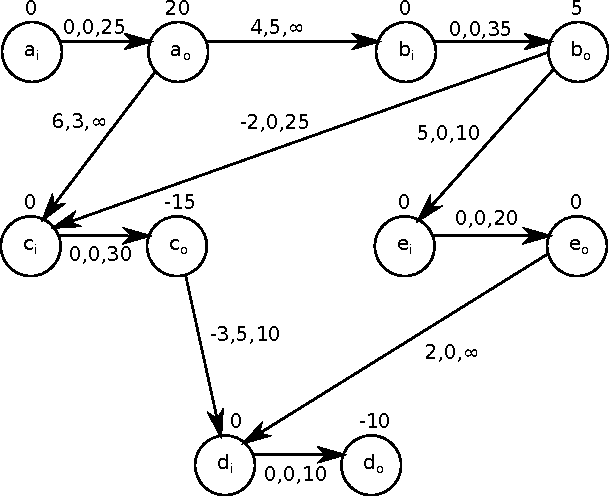
\includegraphics[width=0.7\textwidth]{problem1-step1.pdf}

      Next, we remove lower bounds.  For each arc with a lower bound, we remove
      the lower bound from the source's supply and add it to the destination's
      supply.

      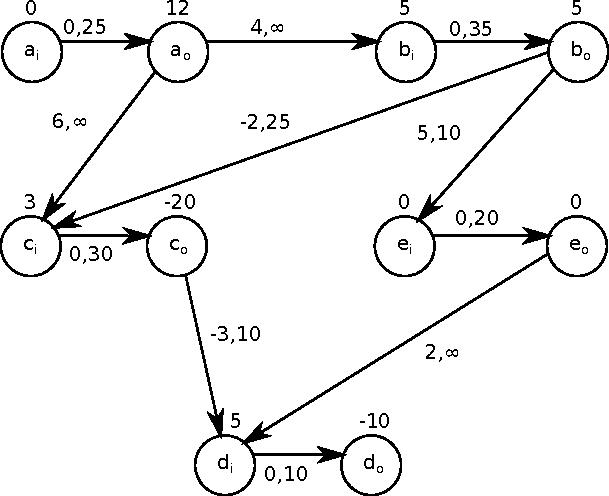
\includegraphics[width=0.7\textwidth]{problem1-step2.pdf}

      Note that here, $a_i$ can never be used.  To simplify, we eliminate it
      during the final step.  In the final step, we eliminate upper bounds.  For
      each arc with an upper bound, we replace it with a node which has a demand
      opposite the upper bound.  The source and destination will both have an
      arc into the new node.  The arc from the source will have the original
      cost, while the arc from the destination to the new node will have cost
      zero.  Finally, we increase the supply in the destination node by the old
      upper bound.  Below is the final result.  Nodes inserted between an
      input and output node are labeled with a subscript $m$ for "middle".
      Nodes inserted along an original node are named $ab$, where $a$ is the
      original source of the arc and $b$ is the original destination.

      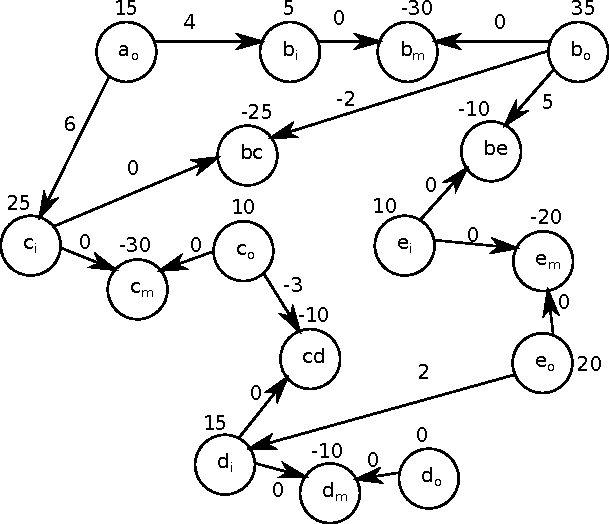
\includegraphics[width=0.7\textwidth]{problem1-step3.pdf}

    \item The flow is drawn below on the original network:

      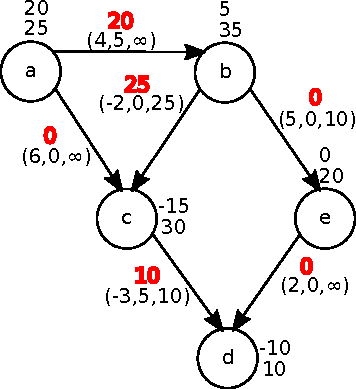
\includegraphics[width=0.5\textwidth]{problem1-partb.pdf}

      Each link is within the upper and lower bounds, and each node has net
      supply of 0.  The flow through $b$ is 20, the flow through $c$ is 25, and
      the flow through $d$ is 10.  So, this flow is feasible.  The residual is:

      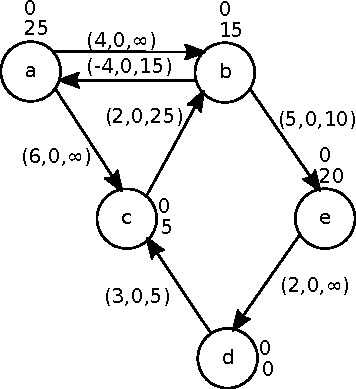
\includegraphics[width=0.5\textwidth]{problem1-partb-resid.pdf}
    \end{enumerate}

    
  \end{problem}

  \begin{problem}{2}
    \begin{question}
      Give an example of a minimum cost network flow problem in which there is
      an optimal solution that is fractional.
    \end{question}

    Since minimum cost network flow is unimodular, there are two ways that a
    fractional solution could exist:

    \begin{enumerate}
    \item The demands are all integer, so there must be an integer optimal
      solution.  However, there could also be a fractional solution that is ``in
      between'' two integer solutions.  Here is an example of such a problem:

      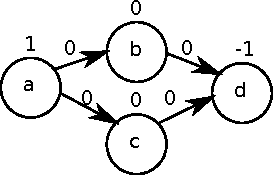
\includegraphics[width=0.4\textwidth]{problem2-eg1.pdf}

      In this example, the fractional solution is to send half a unit through
      $b$, and half a unit through $c$.  This solution can be thought of as ``in
      between'' the two integer solutions (sending all the flow through $b$ or
      through $c$).

    \item The demands are fractional, so there is no integer optimal solution.
      Here is an example of such a problem:

      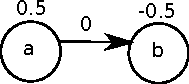
\includegraphics[width=0.3\textwidth]{problem2-eg2.pdf}
    \end{enumerate}
  \end{problem}

  \begin{problem}{3}
    \begin{question}
      Consider the minimum cost network flow problem in problem 1.  Write the
      dual and the complementary slackness conditions.  For simplicity, you are
      allowed to transform the problem into an equivalent one from which the
      dual can be more easily derived.
    \end{question}

    I will use the second intermediate drawing of the MCNF problem I gave in
    problem 1.  This is the drawing where there are costs and upper bounds, but
    no lower bounds or capacities.  This is not exactly the same case as we did
    in class.  In class, we assumed that there were finite upper bounds for each
    arc.  In the case where there is no upper bound, there is simply no
    constraint $-x_{ij} \ge -u_{ij}$ in the primal, and so there is no
    corresponding $\alpha_{ij}$ variable in the dual.  Of course, there are the
    same number of constraints in the dual, just some are missing $\alpha_{ij}$
    variables.  The dual for this problem is given below.  I have included all 0
    coefficients in the objective function for completeness.  Also, I have
    relabeled nodes $a_i, a_o, \dots, e_i, e_o$ to $0, 1, \dots, 8, 9$ for ease
    of translation.

    \begin{alignat*}{1}
      \max 0\pi_0 + 15\pi_1 + 5\pi_2 + 5\pi_3 + 0\pi_4 - 20\pi_5 + 5\pi_6 -
      10\pi7 + 0\pi_8 + 0\pi_9 & \\
      -25\alpha_{01} - 35\alpha_{23} - 25\alpha_{34} - 30\alpha_{45} -
      10\alpha_{38} - 10\alpha_{56} - 20\alpha_{89} - 10\alpha_{67} &\text{
        s.t.} \\
      \pi_0 - \pi_1 - \alpha_{01} &\le 0 \\
      \pi_1 - \pi_2 &\le 4 \\
      \pi_2 - \pi_3 - \alpha_{23} &\le 0 \\
      \pi_0 - \pi_4 &\le 6 \\
      \pi_3 - \pi_4 - \alpha_{34} &\le -2 \\
      \pi_3 - \pi_8 - \alpha_{38} &\le 5 \\
      \pi_4 - \pi_5 - \alpha_{45} &\le 0 \\
      \pi_8 - \pi_9 - \alpha_{89} &\le 0 \\
      \pi_5 - \pi_6 - \alpha_{56} &\le -3 \\
      \pi_9 - \pi_6 &\le 2 \\
      \pi_6 - \pi_7 - \alpha_{67} &\le 0 \\
    \end{alignat*}

    The complementary slackness conditions:

    \begin{align*}
      \alpha_{01} (u_{01} - x_{01}) &= 0 &x_{01} (\pi_0 - \pi_1 - \alpha_{01}) &= 0 \\
                                    &    &x_{12} (\pi_1 - \pi_2 - 4) &= 0 \\          
      \alpha_{23} (u_{23} - x_{23}) &= 0 &x_{23} (\pi_2 - \pi_3 - \alpha_{23}) &= 0 \\
                                    &    &x_{04} (\pi_0 - \pi_4 - 6) &= 0 \\          
      \alpha_{34} (u_{34} - x_{34}) &= 0 &x_{34} (\pi_3 - \pi_4 - \alpha_{34} + 2) &= 0 \\
      \alpha_{38} (u_{38} - x_{38}) &= 0 &x_{38} (\pi_3 - \pi_8 - \alpha_{38} - 5) &= 0 \\
      \alpha_{45} (u_{45} - x_{45}) &= 0 &x_{45} (\pi_4 - \pi_5 - \alpha_{45}) &= 0 \\
      \alpha_{89} (u_{89} - x_{89}) &= 0 &x_{89} (\pi_8 - \pi_9 - \alpha_{89}) &= 0 \\
      \alpha_{56} (u_{56} - x_{56}) &= 0 &x_{56} (\pi_5 - \pi_6 - \alpha_{56} + 3) &= 0 \\
                                    &    &x_{96} (\pi_9 - \pi_6 - 2) &= 0 \\          
      \alpha_{67} (u_{67} - x_{67}) &= 0 &x_{67} (\pi_6 - \pi_7 - \alpha_{67}) &= 0 \\
    \end{align*}
    
  \end{problem}

  \begin{problem}{4}
    \begin{question}
      Consider the minimum cost network flow problem defined on the following
      graph:

      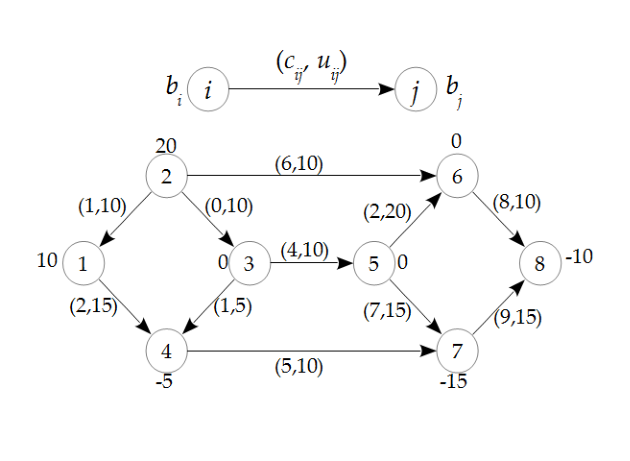
\includegraphics{problem4-network.pdf}

      An optimal solution $x^*$ is:

      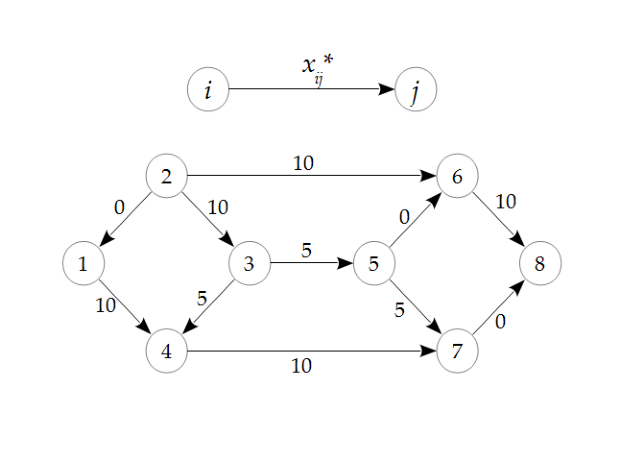
\includegraphics{problem4-flow.pdf}

      In this instance of minimum cost network flow:
      \begin{enumerate}[a.]
        \item Draw the residual network $G(x^*)$.
        \item Specify a set of node potentials $\pi$ that together with $x^*$
          satisfy the reduced cost optimality conditions.  List each arc in the
          residual network and its reduced cost.
        \item Verify that the solution $x^*$ satisfies the complementary
          slackness optimality conditions.  To do so, specify a set of node
          potentials and list the reduced cost of each arc.
      \end{enumerate}
    \end{question}

    \begin{enumerate}[a.]
    \item The residual network is below:

      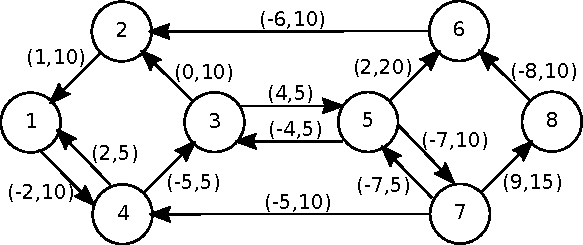
\includegraphics{problem4.pdf}

    \item Below are a set of node potentials:

      \begin{tabular}{ll}
        \hline
        Node & $\pi_i$ \\
        \hline
        1 & 10 \\
        2 & 11 \\
        3 & 11 \\
        4 & 8 \\
        5 & 7 \\
        6 & 5 \\
        7 & 0 \\
        8 & -9 \\
        \hline
      \end{tabular}

      The corresponding reduced costs for each arc:

      \begin{tabular}{llr}
        \hline
        Start & End & $c_{ij}^{\pi}$ \\
        \hline
        1 & 4 & $2-10+8=0$ \\
        2 & 1 & $1-10+10=1$ \\
        3 & 2 & $0-11+11=0$ \\
        3 & 5 & $4-11+7=0$ \\
        4 & 1 & $-2-8+10=0$ \\
        4 & 3 & $-1-8+11=2$ \\
        5 & 3 & $-4-7+11=0$ \\
        5 & 6 & $2-7+5=0$ \\
        5 & 7 & $7-7+0=0$ \\
        6 & 2 & $-6-5+11=0$ \\
        7 & 4 & $-5-0+8=3$ \\
        7 & 5 & $-7-0+7=0$ \\
        7 & 8 & $9-0-9=0$ \\
        8 & 6 & $-8+9+5=6$ \\
        \hline
      \end{tabular}

      All of the reduced costs are $\ge 0$, so this flow satisfies the reduced
      cost optimality condition.

    \item We know that $\alpha_{ij} = \max \{0, -c_{ij}^\pi\}$.  Since all of
      the above $c_{ij}^\pi \ge 0$, we know
      $\alpha_{ij} = 0 \:\: \forall (i,j) \in E$.  Therefore we see that all
      complementary slackness conditions of the form
      $\alpha_{ij}(u_{ij} - x_{ij}) = 0$ are immediately satisfied.  For the
      complementary slackness conditions of the form
      $x_{ij}(c_{ij}^\pi + \alpha_{ij}) = 0$, we have two possibilities:

      \begin{enumerate}[i.]
      \item $c_{ij}^\pi = 0$: for these arcs, we know
        $c_{ij}^\pi + \alpha_{ij} = 0$ so the condition is satisfied.
      \item $c_{ij}^\pi > 0$: for these arcs $c_{ij}^\pi + \alpha_{ij} > 0$, so
        it must be true that $x_{ij} = 0$.  In the table above, we see that the
        arcs corresponding to this case are: $(2,1)$, $(4,3)$, $(7,4)$, and
        $(8,6)$.  We see that for all these arcs, $x_{ij} = 0$ in the original flow.
      \end{enumerate}

      So, both complementary slackness optimality conditions are satisfied.
    \end{enumerate}
  \end{problem}

  \begin{problem}{5}
    \begin{question}
      Two players, called Alice and Bob, play the following game. A set of
      gambling chips are placed on a line. Gambling chips can have arbitrary
      integer values. Then, the players take turn removing one of the chips from
      either end of the remaining line of chips. In other words, at his turn,
      each player removes the chip either at the left or at the right end of the
      line (his choice, but not in the middle) and places it in his collection.
      The player with the larger total value wins.

      \begin{enumerate}[a.]
      \item Show an arrangement of gambling chips where Alice would lose if she
        always picked the end-of-line chip with the largest possible value.
      \item Design an algorithm that takes as input a linear arrangement of
        chips and that returns Alice's best strategy assuming that Bob will make
        the most of the remaining chip arrangement. Your algorithm should
        formulate the game as a shortest path problem.  
      \item Determine the running time of your algorithm assuming that shortest
        paths are computed with Dijkstra's algorithm. Suggest an improvement to
        the shortest path computation that results in a faster run time.
      \end{enumerate}
    \end{question}

    \begin{enumerate}[a.]
    \item One such arrangement of chips would be:
      $1, 6, 7, 5, 8, 4, 9, 3, 10, 2$.  Assuming Alice goes first, her total
      would be $2 + 3 + 4 + 5 + 1 = 15$, while Bob would have
      $10 + 9 + 8 + 7 + 1 = 35$.
    \item If we define the objective function as the difference between your
      score and your opponent's score, then the best strategy when given a
      sequence $A$ of chip values and starting and ending point $i$ and $j$
      respectively can be defined recursively:

      \begin{equation*}
        Strategy(A,i,j) = \max \{A[i] - Strategy(A,i+1,j), A[j] - Strategy(A,i,j+1)\}
      \end{equation*}

      The base case, of course, is when $i=j$, at which point
      $Strategy(A,i,i)=A[i]$.  We can then create a graph out of this, where
      there is a node $(i,j)$ if $i <= j$.  For each node $(i,j)$, there is an
      edge connecting it to $(i-1, j)$ and $(i,j-1)$, having a cost with
      magnitude of $A[i]$ and $A[j]$ respectively.  The sign of the cost is
      determined by whether $i + (n-j)$ is even, where $n$ is the number of
      chips in the sequence.  If $i+(n-j)$ is even, the sign is negative,
      otherwise, positive.  The shortest path from node $(0,n)$ to any end node
      $(i,i)$ is Alice's strategy.

      So, the algorithm is simply to construct this graph and find the above
      shortest path.

    \item We cannot use Dijkstra's Algorithm because of the negative weight
      edges in the graph.  If we added a suitable constant to every edge, the
      weights would be non-negative and therefore we could apply Dijkstra's
      Algorithm.  This would give us a runtime of $O(n^2 + n^2 \log{n^2})$
      (where $n$ is the number of chips).  We would be better off simply filling
      out a table of the above strategy function instead of using a search
      algorithm.  This would improve our runtime to $O(n^2)$.
      
    \end{enumerate}
  \end{problem}

  \begin{problem}{7}
    \begin{question}
      Consider problem 5 in Homework Assignment 2. Show that the linear program
      is equivalent to a minimum cost network flow problem and prove that this
      program has always an integer optimal solution.

      \textbf{Problem 5 from Homework Assignment 2:}

      \begin{align*}
        \min x_1 + x_2 + 3x_3 + 2x_4 + 4x_5 & \\
        \text{s.t. } x_1 + x_3 + x_5 &= 2 \\
        x_4 - x_3 &= 1 \\
        x_2 - x_1 &= -1 \\
        x_2 + x_4 + x_5 &= 2 \\
        0 \le x_1 &\le 1 \\
        0 \le x_2 &\le 2 \\
        0 \le x_3 &\le 1 \\
        0 \le x_4 &\le 3 \\
        0 \le x_5 &\le 2 \\
      \end{align*}
    \end{question}

    When a Minimum Cost Network Flow problem is expressed as a Linear Program,
    its form is:

    \begin{alignat*}{2}
      \min \sum_{(i,j) \in E} c_{ij} x_{ij} &\: \text{ s.t.} && \\
      \sum_{j: (i,j) \in E} x_{ij} - \sum_{j: (j,i) \in E} x_{ji} &= b_i &\forall i \in V&\\
      0 \le x_{ij} &\le u_{ij} & \forall (i,j) \in E &
    \end{alignat*}

    Each variable in the LP corresponds to an arc.  Each constraint corresponds
    to a node.  A positive sign in a constraint means it is outgoing, while a
    negative sign in a constraint means it is incoming.  Each variable should
    then occur twice in the constraints, once with a positive sign, and once
    with a negative sign.  If we negate everything in the fourth constraint, we
    can see that the given LP is exactly in that form.  We will call the nodes 1
    through 4 in the same order the constraints are given above.  Then we have
    the following table of variables and their corresponding arcs;

    \begin{tabular}{llll}
      \hline
      Var & Arc & Cost & Upper \\
      \hline
      $x_1$ & $(1,3)$ & 1 & 1 \\
      $x_2$ & $(3,4)$ & 1 & 2 \\
      $x_3$ & $(1,2)$ & 3 & 1 \\
      $x_4$ & $(2,4)$ & 2 & 3 \\
      $x_5$ & $(1,4)$ & 4 & 2 \\
      \hline
    \end{tabular}

    The nodes have supplies given by the right hand side of their corresponding
    constraints.  The table below provides those $b_i$ values.

    \begin{tabular}{ll}
      \hline
      Constraint & $b_i$ \\
      \hline
      1 & 2 \\
      2 & 1 \\
      3 & -1 \\
      4 & -2 \text{ (due to negated constraint)} \\
      \hline
    \end{tabular}

    In class, we proved that MCNF problems are unimodular.  Therefore, since the
    $b_i$ in this problem are all integer, there must be an optimal basic
    feasible solution which is integer.
  \end{problem}

\end{document}